\section{Results}
\label{sec:results}

Figures~\ref{fig:T21bHT2bHExpObs500800}-\ref{fig:T21bHT2bH1dSignif}
contain the results of the reinterpretation of the CMS data for both models.
To show how well signal model A agrees with the excess observed by CMS,
Fig.~\ref{fig:T21bHT2bHExpObs500800} (top) displays the expected SM background
distribution and uncertainty taken from the CMS result compared to the distribution of the
signal events for $m_{\sbottom_2}=500\GeV$ and
$m_{\sbottom_2}=800\GeV$, with other mass parameters set as
$m_{\sbottom_2}=130\GeV$, $m_{\chiztwo}=230\GeV$, and
$m_{\chizone}=100\GeV$. The bin numbers correspond to the order of the
signal regions in the yield tables in Ref.~\cite{RazorHgaga} and are
reproduced in Tab.~\ref{tab:bins}.
\begin{table}[htb] \centering
\caption{\label{tab:bins}\texttt{HighRes} bin numbering scheme as in Ref.~\cite{RazorHgaga}.}
\begin{tabular}{c|cc}
\hline\hline
Bin &$\MR$ range & $\Rtwo$ range \\
\hline
 0 & $ [150, 250]$ & $[0.00, 0.05]$\\
 1 & $[150, 250]$ & $[0.05, 0.10]$\\
 2 & $[150, 250]$ & $[0.10, 0.15]$\\
 3 &  $[150, 250]$ & $[0.15, 1.00]$\\
 4 &  $[250, 400$ & $[0.00, 0.05]$\\
 5 &  $[250, 400]$ & $[0.05, 0.10]$\\
 6 &  $[250, 400]$ & $[0.10, 1.00]$\\
 7 & $[400, 1400]$ & $[0.00, 0.05]$\\
8 &  $[400, 1400]$ & $[0.05, 1.00]$\\
 9 & $[1400, 3000]$ & $[0.00, 1.00]$\\
\hline\hline
\end{tabular}
\end{table}
The normalization for each signal model is taken from the mode (i.e. ``best-fit'') signal cross section of the posterior density in the
\texttt{HighRes} box. Fig.~\ref{fig:T21bHT2bH1dLimit} (top), shows the
95\% CL combined upper limit on the cross section for model A. Finally,
Fig.~\ref{fig:T21bHT2bH1dSignif} (top) shows the maximum significance
$Z$ as well as the best fit signal cross section for model A as a function of $m_{\sbottom_2}$.

The bottom of Fig.~\ref{fig:T21bHT2bHExpObs500800}-\ref{fig:T21bHT2bH1dSignif} are
the analogous results for model B. The chosen model B mass points in Fig.~\ref{fig:T21bHT2bHExpObs500800} are
$m_{\sbottom_1}=500\GeV$ or $m_{\sbottom_1}=800\GeV$, $m_{\chiztwo}=230\GeV$, and
$m_{\chizone}=100\GeV$. The limit and significance scans in
Fig.~\ref{fig:T21bHT2bH1dLimit}~and~\ref{fig:T21bHT2bH1dSignif} are
performed as a function of the $\sbottom_1$ mass. For model B, we also
compare both the excluded cross section at 95\% CL and the best-fit cross section
as a function of the $\sbottom_1$ mass to the NLO$+$NLL predicted cross section at
$\sqrt{s}=8\TeV$~\cite{NLONLL1,NLONLL2,NLONLL3,NLONLL4,NLONLL5,Borschensky:2014cia}. We
find the $8\TeV$ data excludes bottom squark pair prodction below $m_{\sbottom_1}=330\GeV$ for
the chosen neutralino masses of $m_{\chiztwo}=230\GeV$ and
$m_{\chizone}=100\GeV$. More interestingly, the largest combined significance
is $1.8\sigma$ for $m_{\sbottom_1}=500\GeV$ and the best-fit cross section
is $0.4\unit{pb}$, which is of the same order of magnitude as the
predicted cross section.

\begin{figure}[htb]\centering
\begin{tabular}{c}
\subfigure{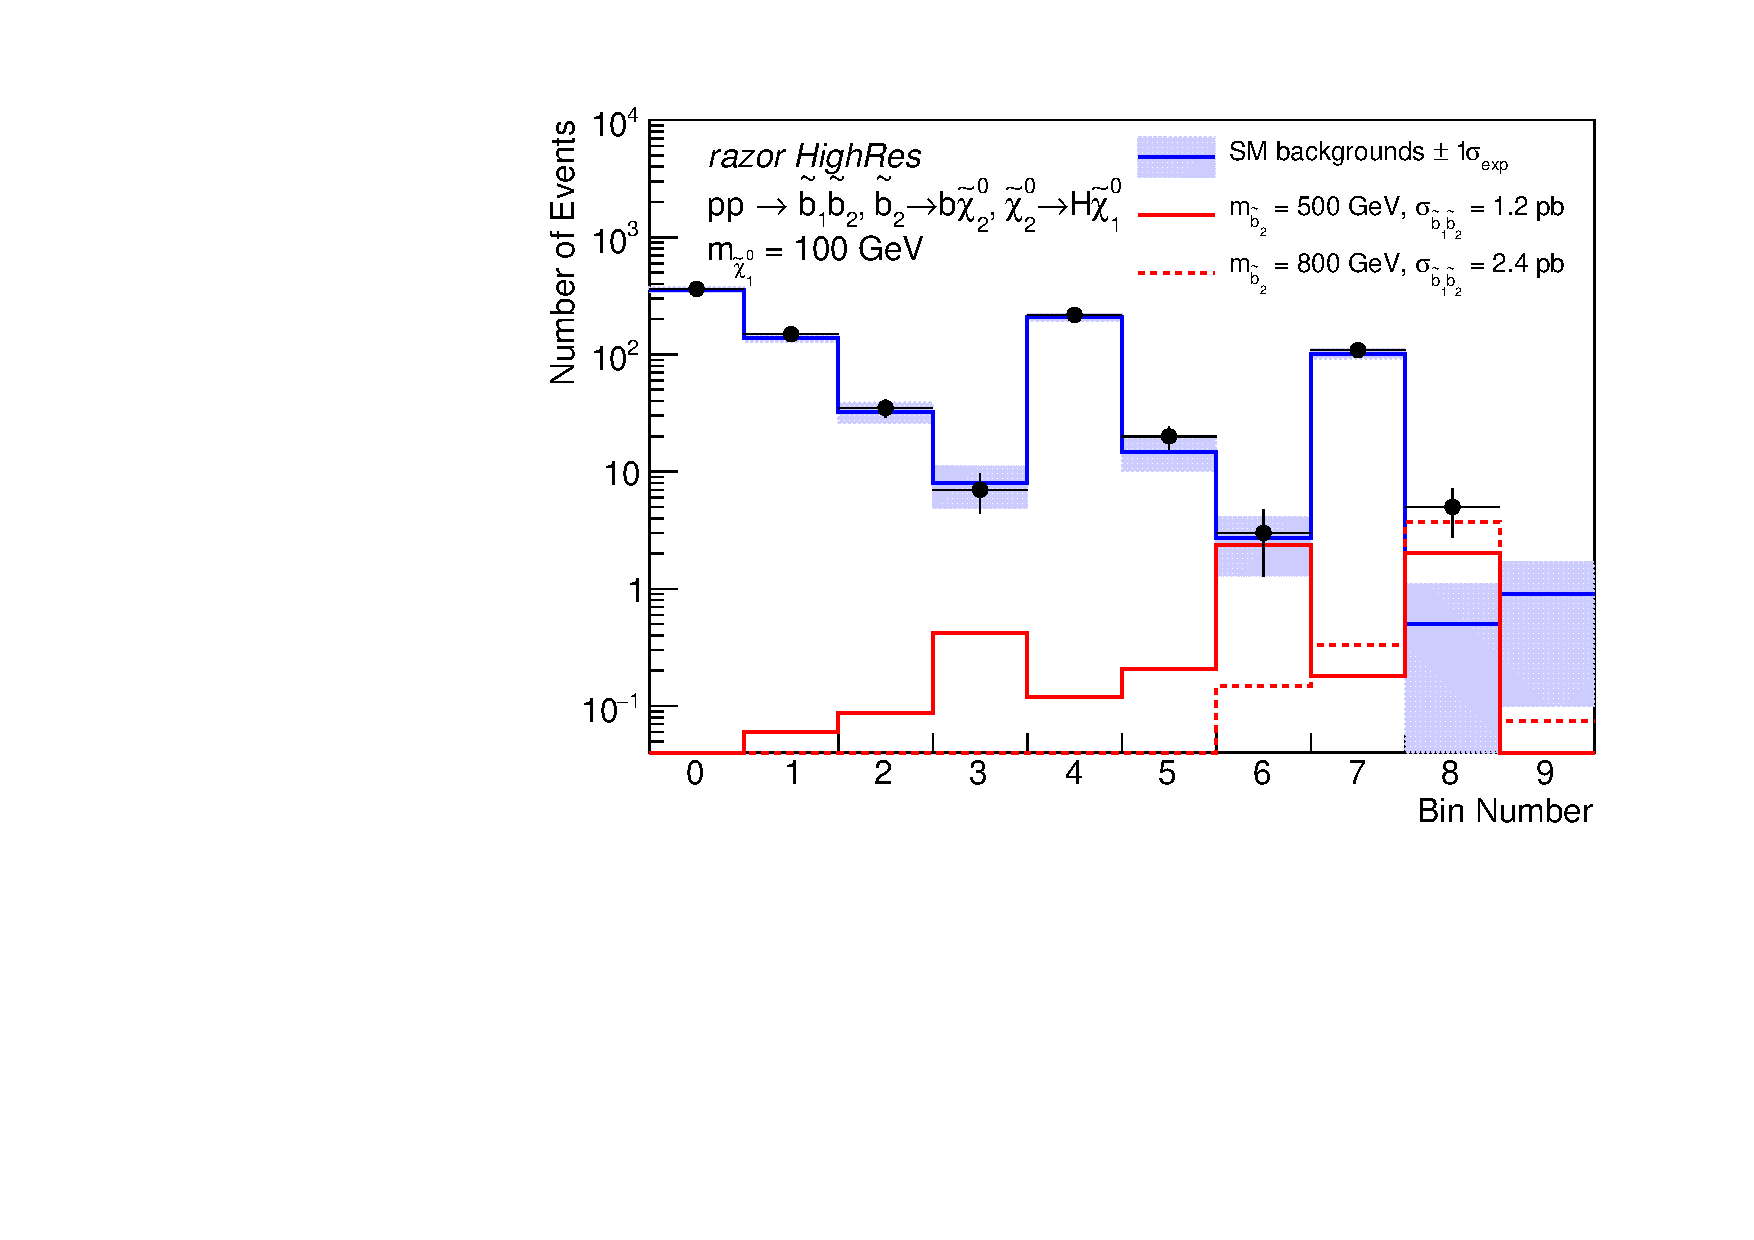
\includegraphics[width=0.45\textwidth]{plots/obsexp_T21bH_HighRes.pdf}}\\
\subfigure{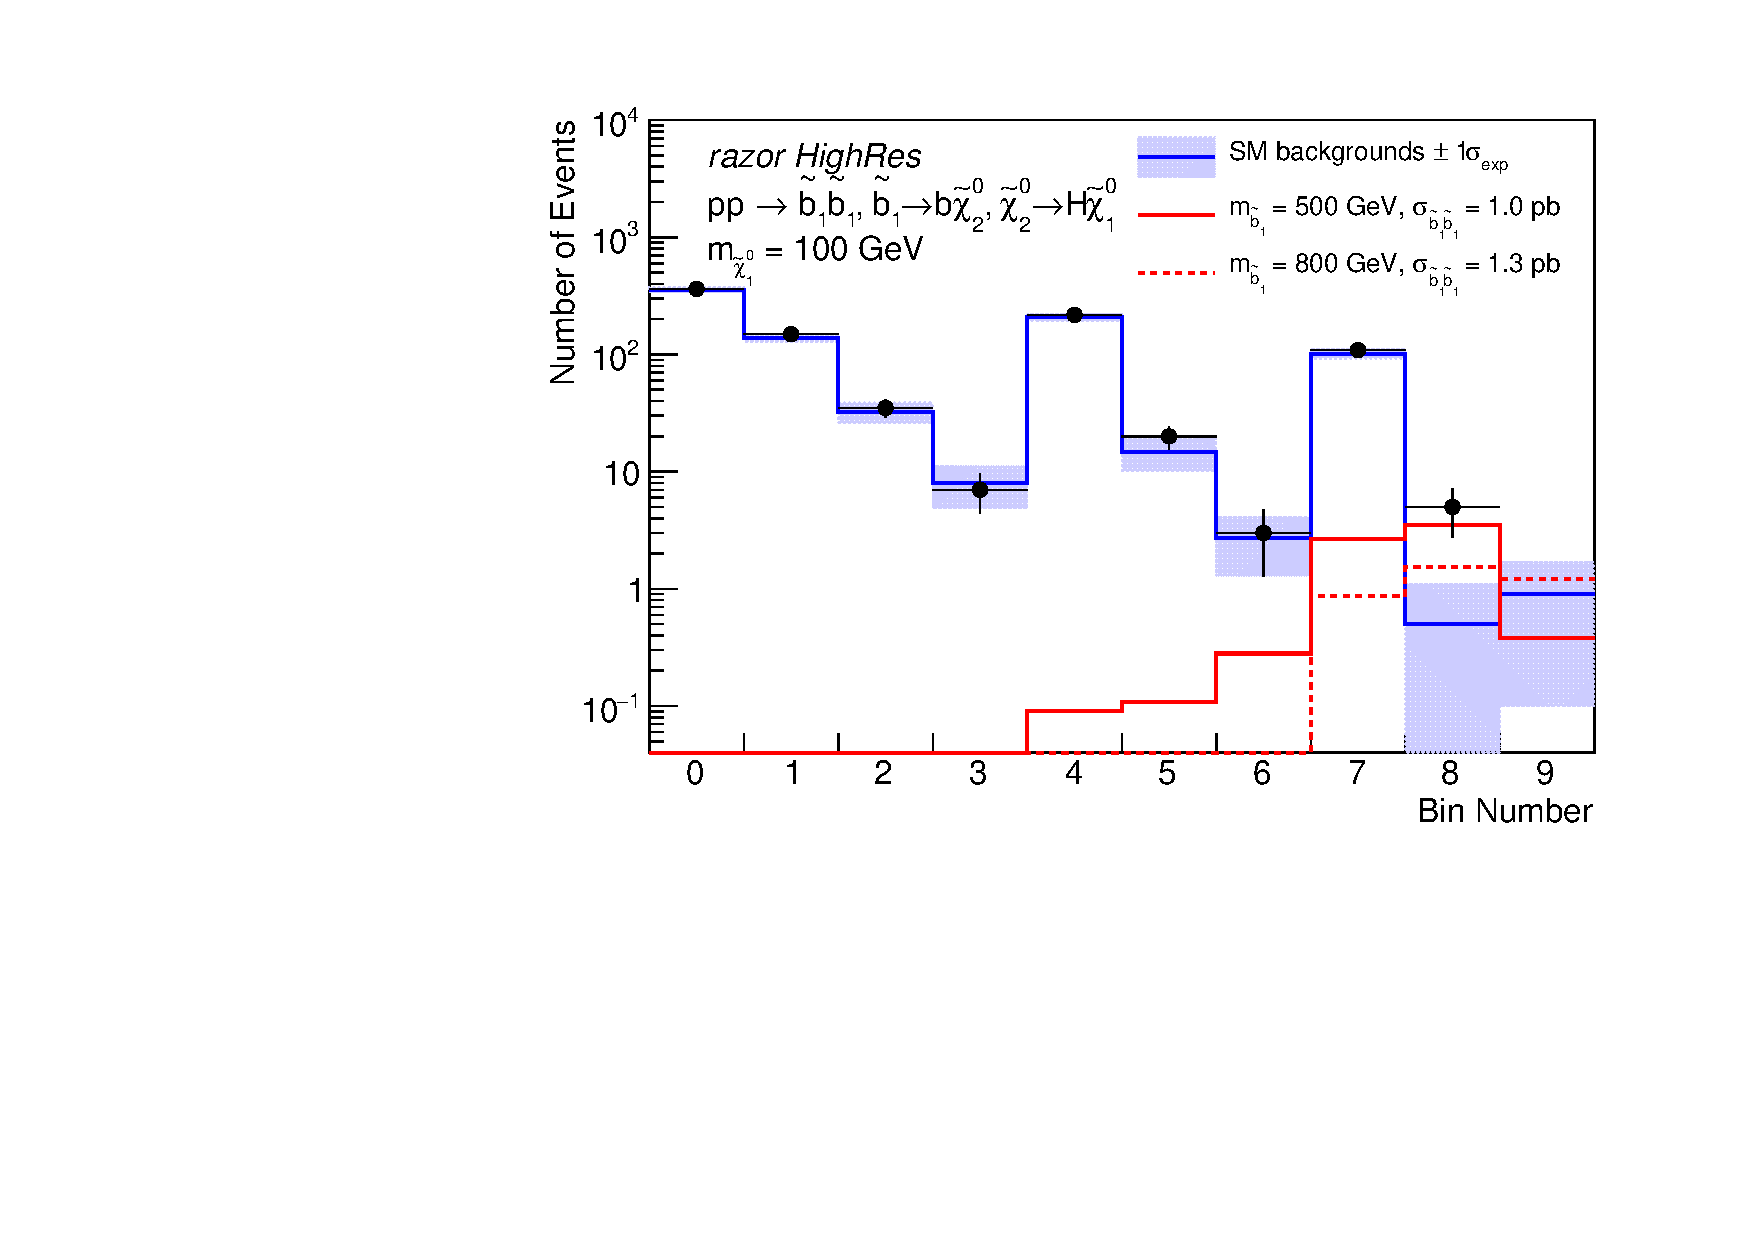
\includegraphics[width=0.45\textwidth]{plots/obsexp_T2bH_HighRes.pdf}}
\end{tabular}
\caption{\label{fig:T21bHT2bHExpObs500800} (Top) The expected background and
  uncertainty (multiplied by a factor of two as explained in the text) compared to the best-fit signal distribution in the \texttt{HighRes} box for two particular
  mass points, $m_{\sbottom_2}=500\GeV$ and $m_{\sbottom_2}=800\GeV$,
  in model A. (Bottom) The expected background and
  uncertainty (multiplied by a factor of two as explained in the text) compared to the best-fit signal distribution in the \texttt{HighRes} box for two particular
  mass points, $m_{\sbottom_1}=500\GeV$ and $m_{\sbottom_1}=800\GeV$,
  in model B. The bin numbers correspond to the order of the signal regions in the yield tables in Ref.~\cite{RazorHgaga} and are reproduced in Tab.~\ref{tab:bins}.}
\end{figure}

\begin{figure}[htb]\centering
\subfigure{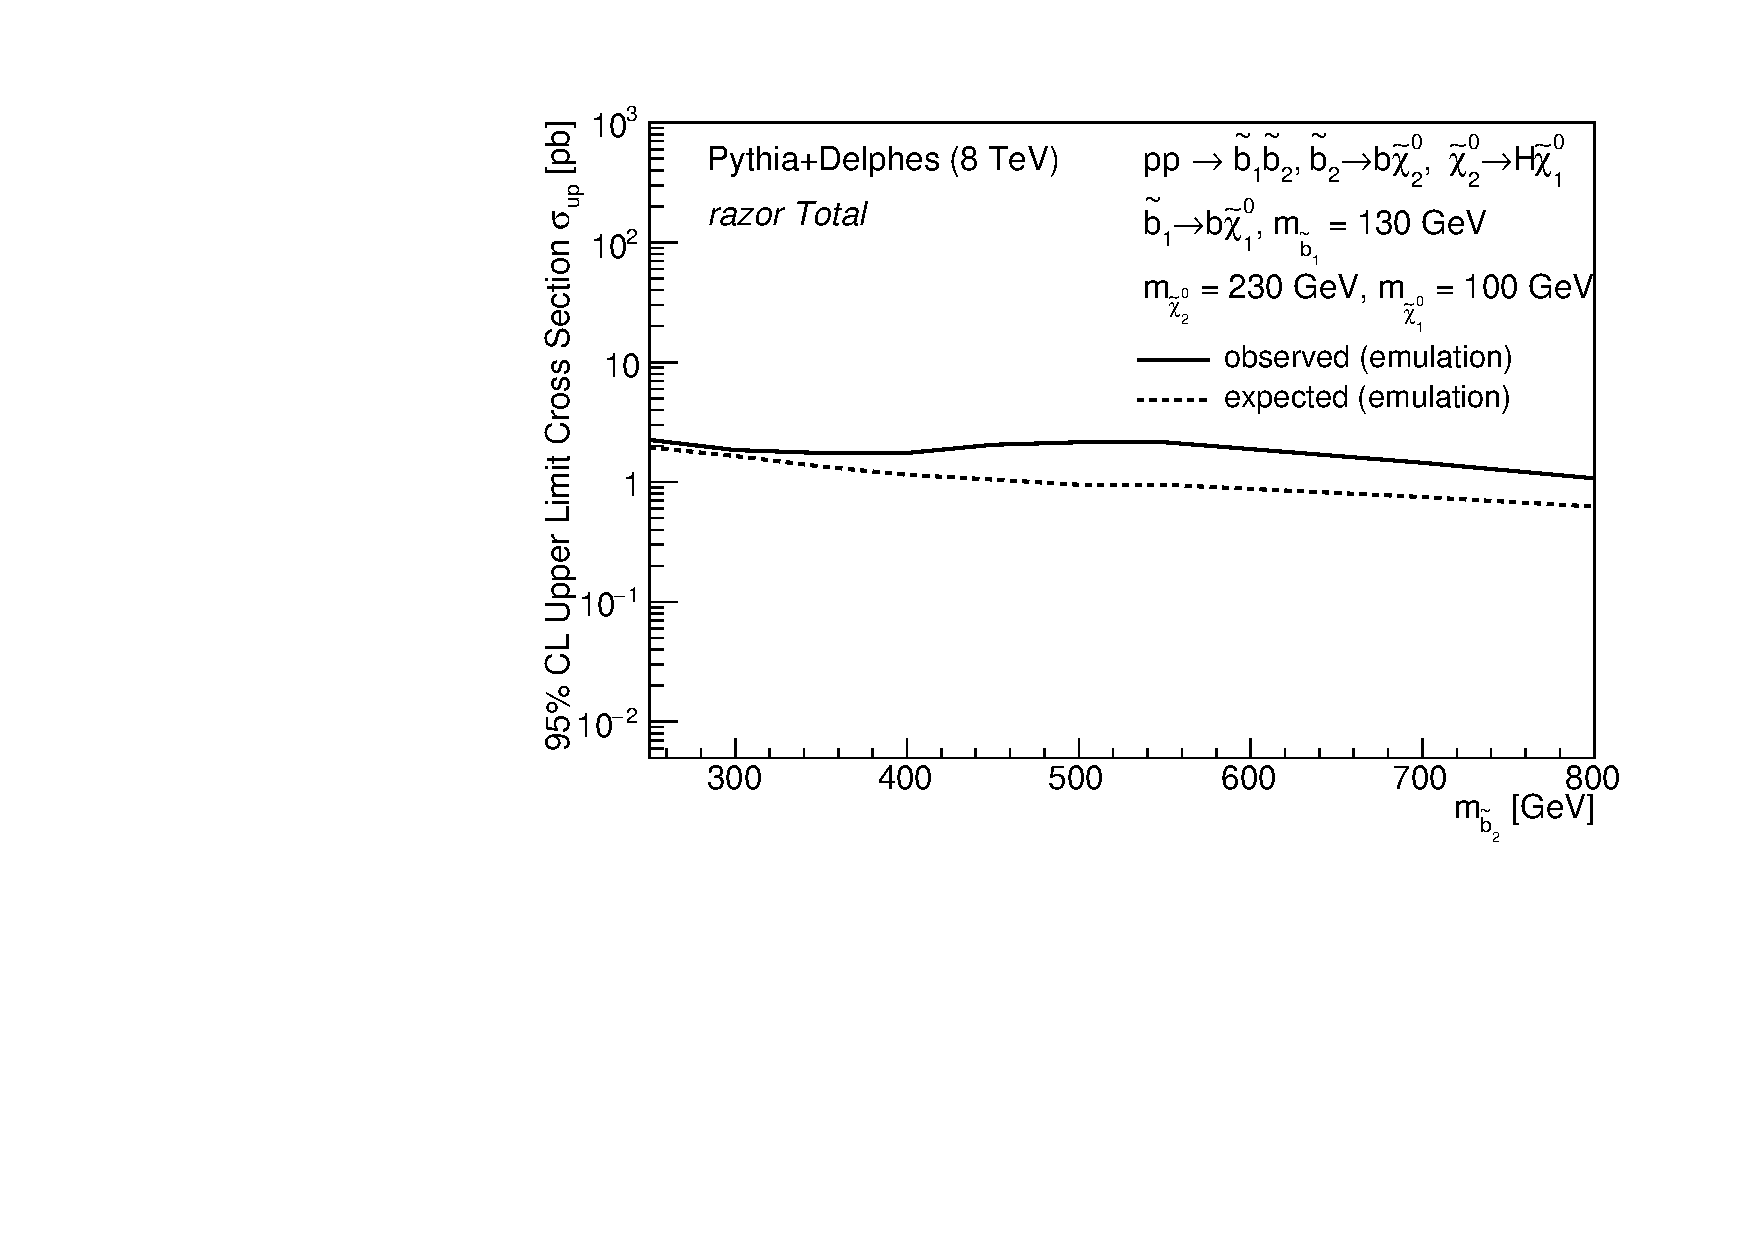
\includegraphics[width=0.45\textwidth]{plots/xsecUL_T21bH_130_100_Total.pdf}}\\
\subfigure{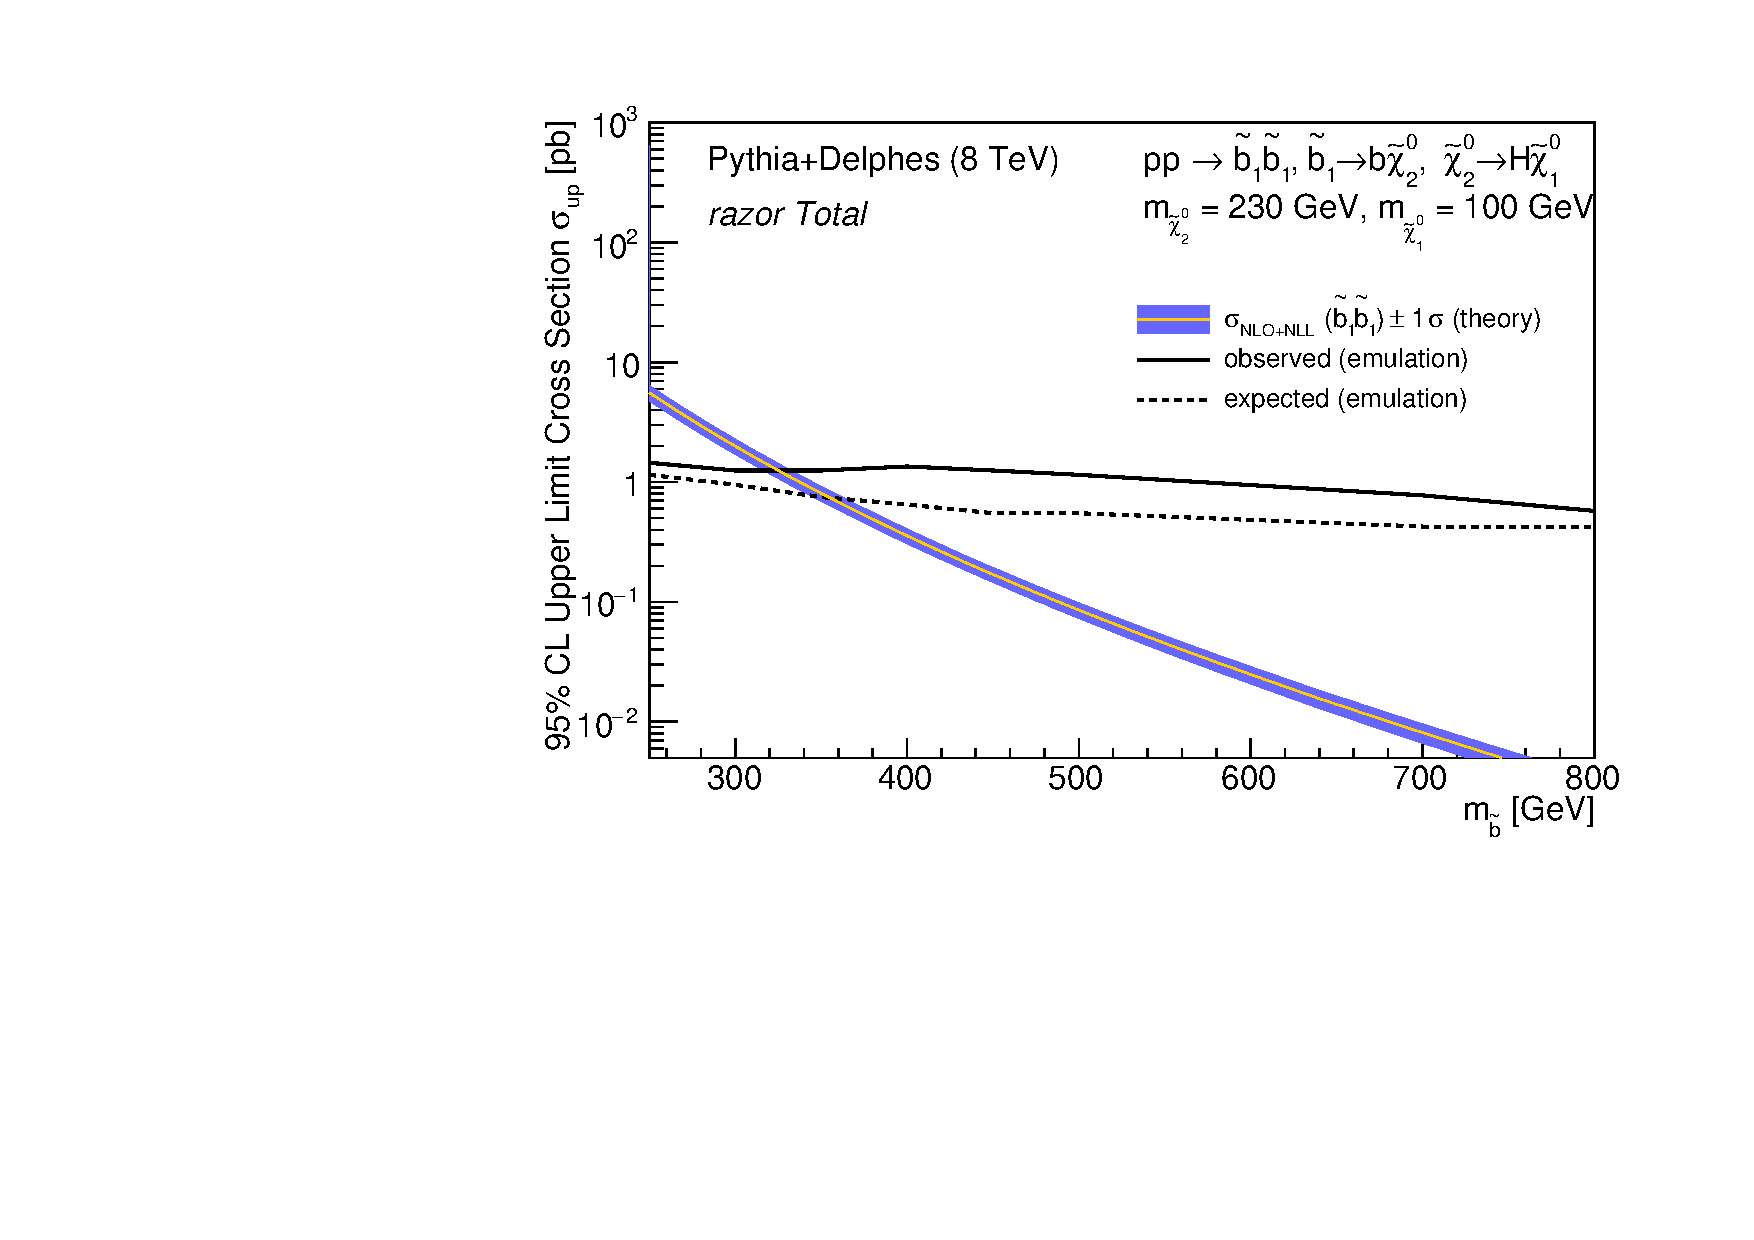
\includegraphics[width=0.45\textwidth]{plots/xsecUL_T2bH_100_Total.pdf}}
\caption{\label{fig:T21bHT2bH1dLimit} (Top) The 95\% CL upper limit on the
  cross section on $\sbottom_1\sbottom_2$ production in model A as a function of $m_{\sbottom_2}$ (black). (Bottom) The 95\% CL upper limit on the
  cross section on $\sbottom_1\sbottom_1$ production in model B as a function of $m_{\sbottom_1}$ (black) compared
  to the NLO+NLL predicted cross section (yellow). Note, these scans assume
  $m_{\chiz_1}=100\GeV$, $m_{\chiz_2}=230\GeV$, and for model A $m_{\sbottom_1}=130$\GeV. }
\end{figure}

\begin{figure}[htb]\centering
\subfigure{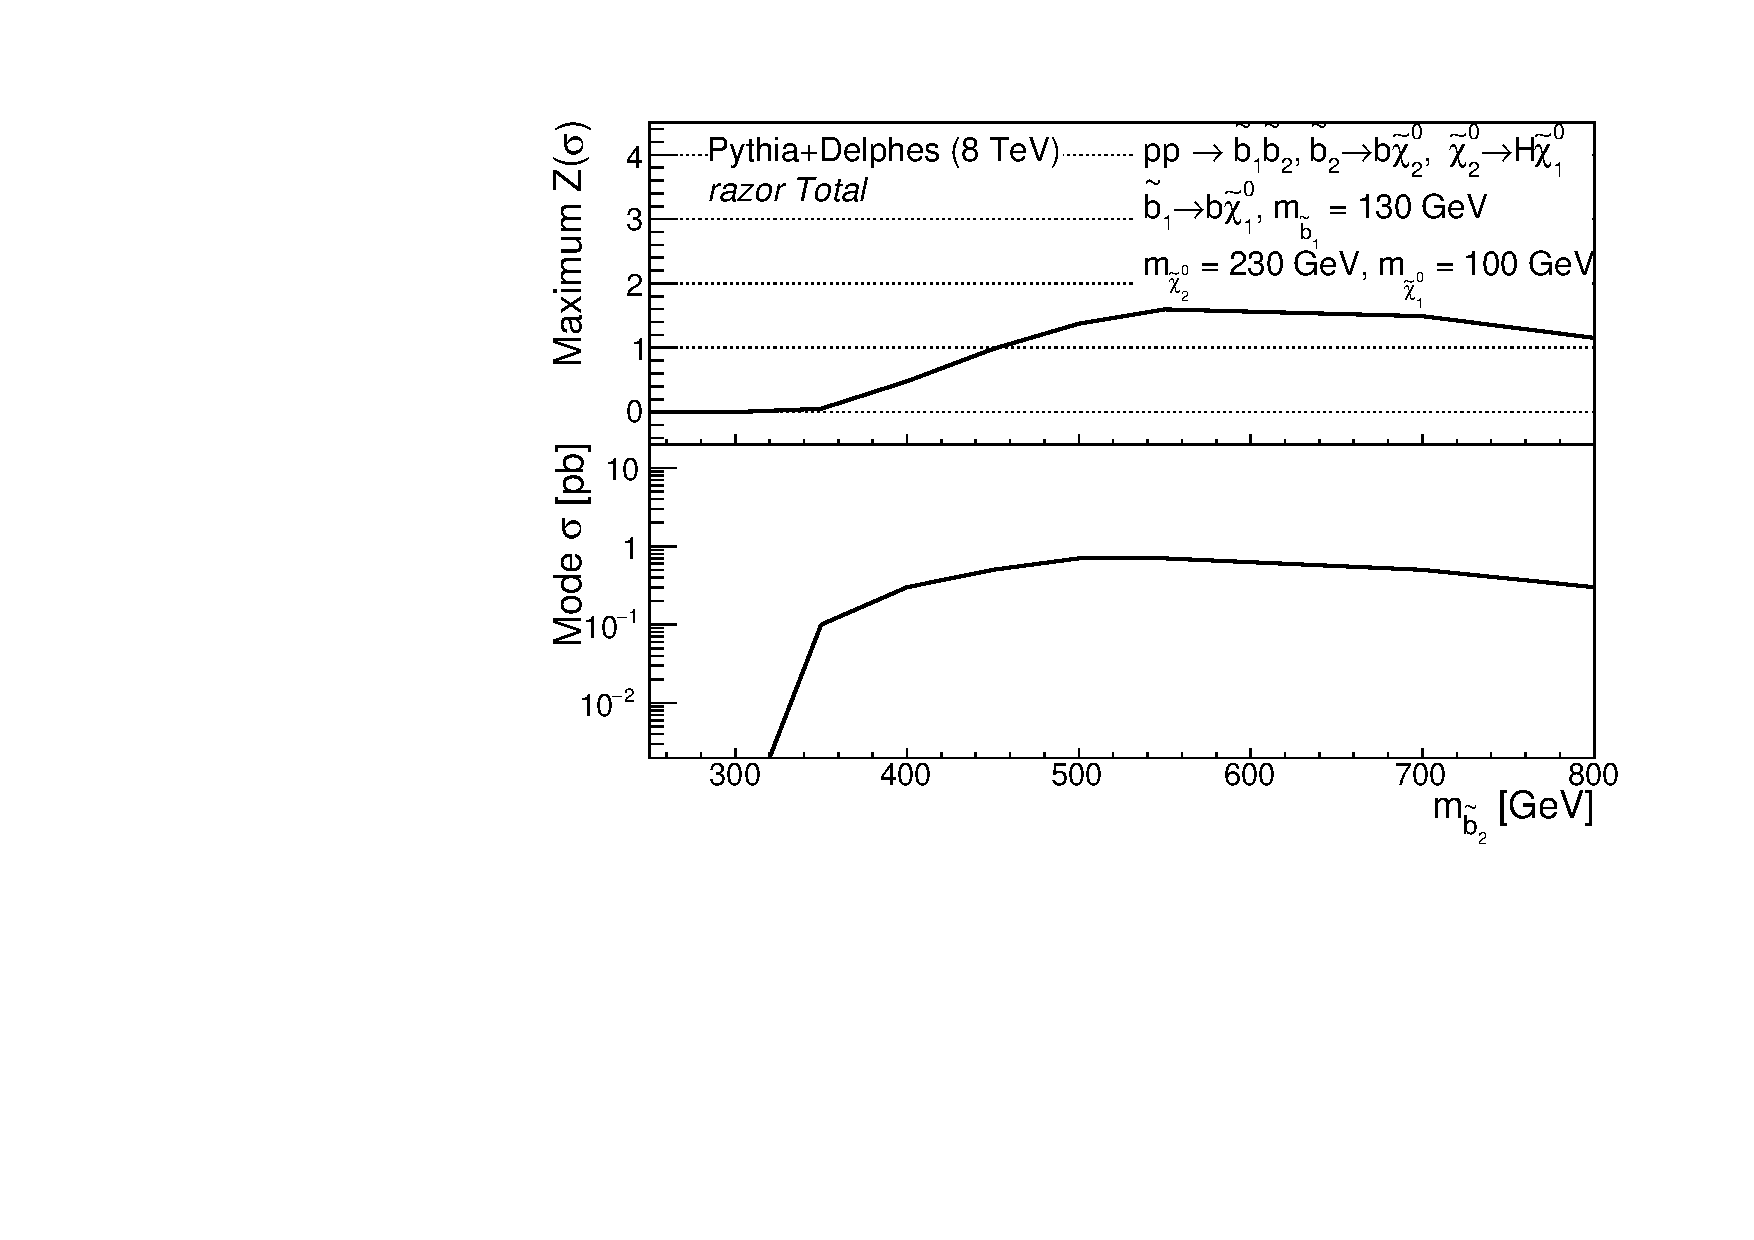
\includegraphics[width=0.45\textwidth]{plots/signif_T21bH_130_100_Total.pdf}}\\
\subfigure{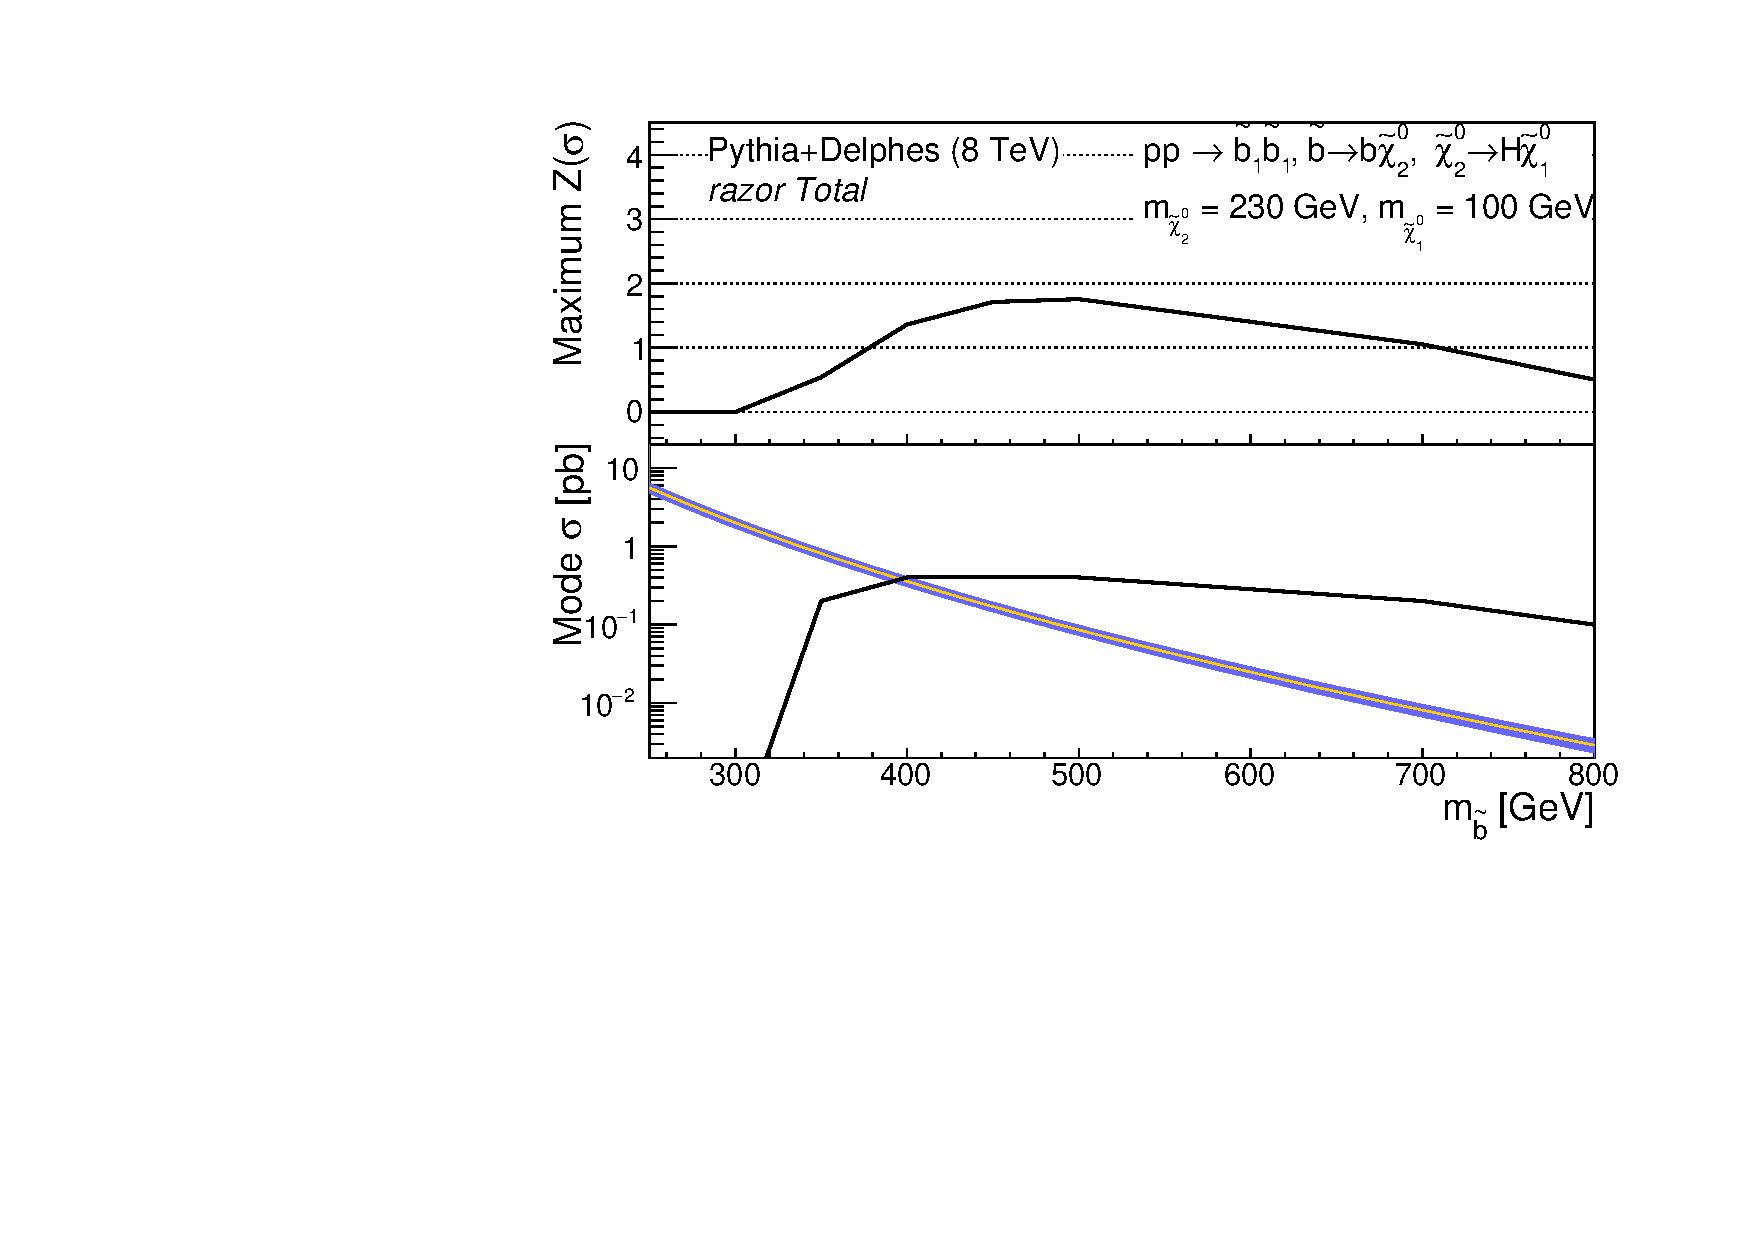
\includegraphics[width=0.45\textwidth]{plots/signif_T2bH_100_Total.pdf}}
\caption{\label{fig:T21bHT2bH1dSignif} (Top) The maximum significance $Z(\sigma)$ for a
  given $m_{\sbottom_2}$ in the top panel and the ``best fit'' signal cross
  section $\sigma$ in the bottom panel for model A.  (Bottom) The maximum significance $Z(\sigma)$ for a
  given $m_{\sbottom_1}$ in the top panel and the ``best fit'' signal cross
  section $\sigma$ in the bottom panel for model B.  Note, these scans assume
  $m_{\chiz_1}=100\GeV$, $m_{\chiz_2}=230\GeV$, and for model A $m_{\sbottom_1}=130$\GeV.}
\end{figure}
